\section{Daredevil y su astigmatismo (1 pt)}

Daredevil está muy preocupado con la situación de la salud en el país, ya que le dijeron que mientras más ciego esté,  más fila le toca hacer para reclamar los medicamentos para la ceguera. Dado que él no está seguro del porcentaje de miopía y astigmatismo que presenta, decide pedir una cita con el oftanmólogo. Sin embargo, se la dieron para septiembre. El Punisher le dice entonces que la única forma de lograr la cita rápido, es armando un "mierdero" en la EPS, pero éste se rehúsa a armarlo; en su lugar, investiga en ChatGPT cuál sería la fórmula para calcular el porcentaje de miopía y astigmatismo de una persona. La IA le arroja la siguiente expresión:

\[
f(x) \;=\; \frac{A\times 10^{-2}}{8} \,\cos\bigl(x \;-\; A\times 10^{-3}\bigr) \;-\; x,
\]
siendo \(x \times 100\%\) el porcentaje de miopía y astigmatismo de la persona, y \(A\) corresponde a 510. El problema se reduce a resolver \(f(x) = 0\).

\subsection{Ayude al Diablo}

Ayude  al Diablo a calcular su porcentaje de ceguera, usando $510$, y el
método de punto fijo con una tolerancia de 6 cifras significativas, y una
condición inicial $x_0 = 0$. Note que $g(x) = f(x) - x$.
Dé una respuesta al Diablo, y entregue la tabla solución en el formato visto en clase.

Sea la función dada:
\[
f(x) \;=\; \frac{A\times10^{-2}}{8}\,\cos\bigl(x - A\times10^{-3}\bigr)\;-\;x
\quad\text{con}\quad A=510.
\]
La raíz de la ecuación \(f(x)=0\) proporciona \(x \times 100\%\) como porcentaje de miopía y astigmatismo.

\subsection{Aplicación del método de punto fijo}

Para \(A = 510\),
\[
A\times 10^{-2} \;=\; 5.1,
\quad
\frac{5.1}{8} \;=\; 0.6375,
\quad
A\times 10^{-3} \;=\; 0.510.
\]
Por lo tanto, la función de iteración es
\[
g(x) \;=\; 0.6375 \,\cos\bigl(x \;-\; 0.510\bigr).
\]
Con \(x_0 = 0\) y tolerancia \(10^{-6}\), se ejecuta:
\[
x_{n+1} \;=\; g(x_n) \;=\; 0.6375 \,\cos\bigl(x_n - 0.510\bigr).
\]

\subsection{Tabla de iteraciones}

A continuación, se muestra la tabla generada (formato \texttt{long} en \textsc{Matlab}). En cada paso se listan: el índice \(n\), la aproximación \(x_n\), el valor \(f(x_n)\) y el error.

\[
\begin{array}{c|c|c|c}
\toprule
\textbf{n} 
& x_n 
& f(x_n)\;=\;\dfrac{A\times10^{-2}}{8}\cos(x_n - A\times 10^{-3}) - x_n
& Error \\
\midrule
0 & 0.000000000000000 & 0.556374623624166 & 1.000001000000000 \\[6pt]
1 & 0.556374623624166 & 0.080439993649312 & 0.556374623624166 \\[6pt]
2 & 0.636814617273478 & -0.004433871777047 & 0.080439993649312 \\[6pt]
3 & 0.632380745496431 & 0.000351276126239 & 0.004433871777047 \\[6pt]
4 & 0.632732021622670 & -0.000027376443341 & 0.000351276126239 \\[6pt]
5 & 0.632704645179329 & 0.000002136367937 & 0.000027376443341 \\[6pt]
6 & 0.632706781547266 & -0.000000166698095 & 0.000002136367937 \\[6pt]
7 & 0.632706614849171 & 0.000000013007346 & 0.000000166698095 \\
\bottomrule
\end{array}
\]

En la iteración \(n=7\), se logra un error menor que \(10^{-6}\). Por tanto, la aproximación final con 6 cifras significativas es

\[
x \;\approx\; 0.632707.
\]

\subsection{Resultado Final}

Puesto que la fracción \(x\) multiplicada por 100\% indica el porcentaje de miopía y astigmatismo, se concluye:
\[
\boxed{
\text{Porcentaje de ceguera} 
\;\approx\; 63.2707\%.
}
\]

Con la presición solicitada ($63.2707\%$) parece que el Diablo a duras penas va
a poder ver la fila en la EPS.

\section{Análisis Gráfico (1 pt)}

El Diablo no creía en este método, sin embargo ha encontrado una solución con
el mismo. Explique gráficamente porque se encontró una solución, verificando si
la función $g(x)$ cumple los criterios del teorema de punto fijo en el intervalo
$[0, 2]$, para ser una buena función. (Verifique los tres criterios). Entregue su procedimiento y respuesta. 

\subsection{Gráfico de $f(x)$ y $g(x)$}
\begin{figure}[H]
    \centering
    \begin{subfigure}[b]{\textwidth}
        \centering
        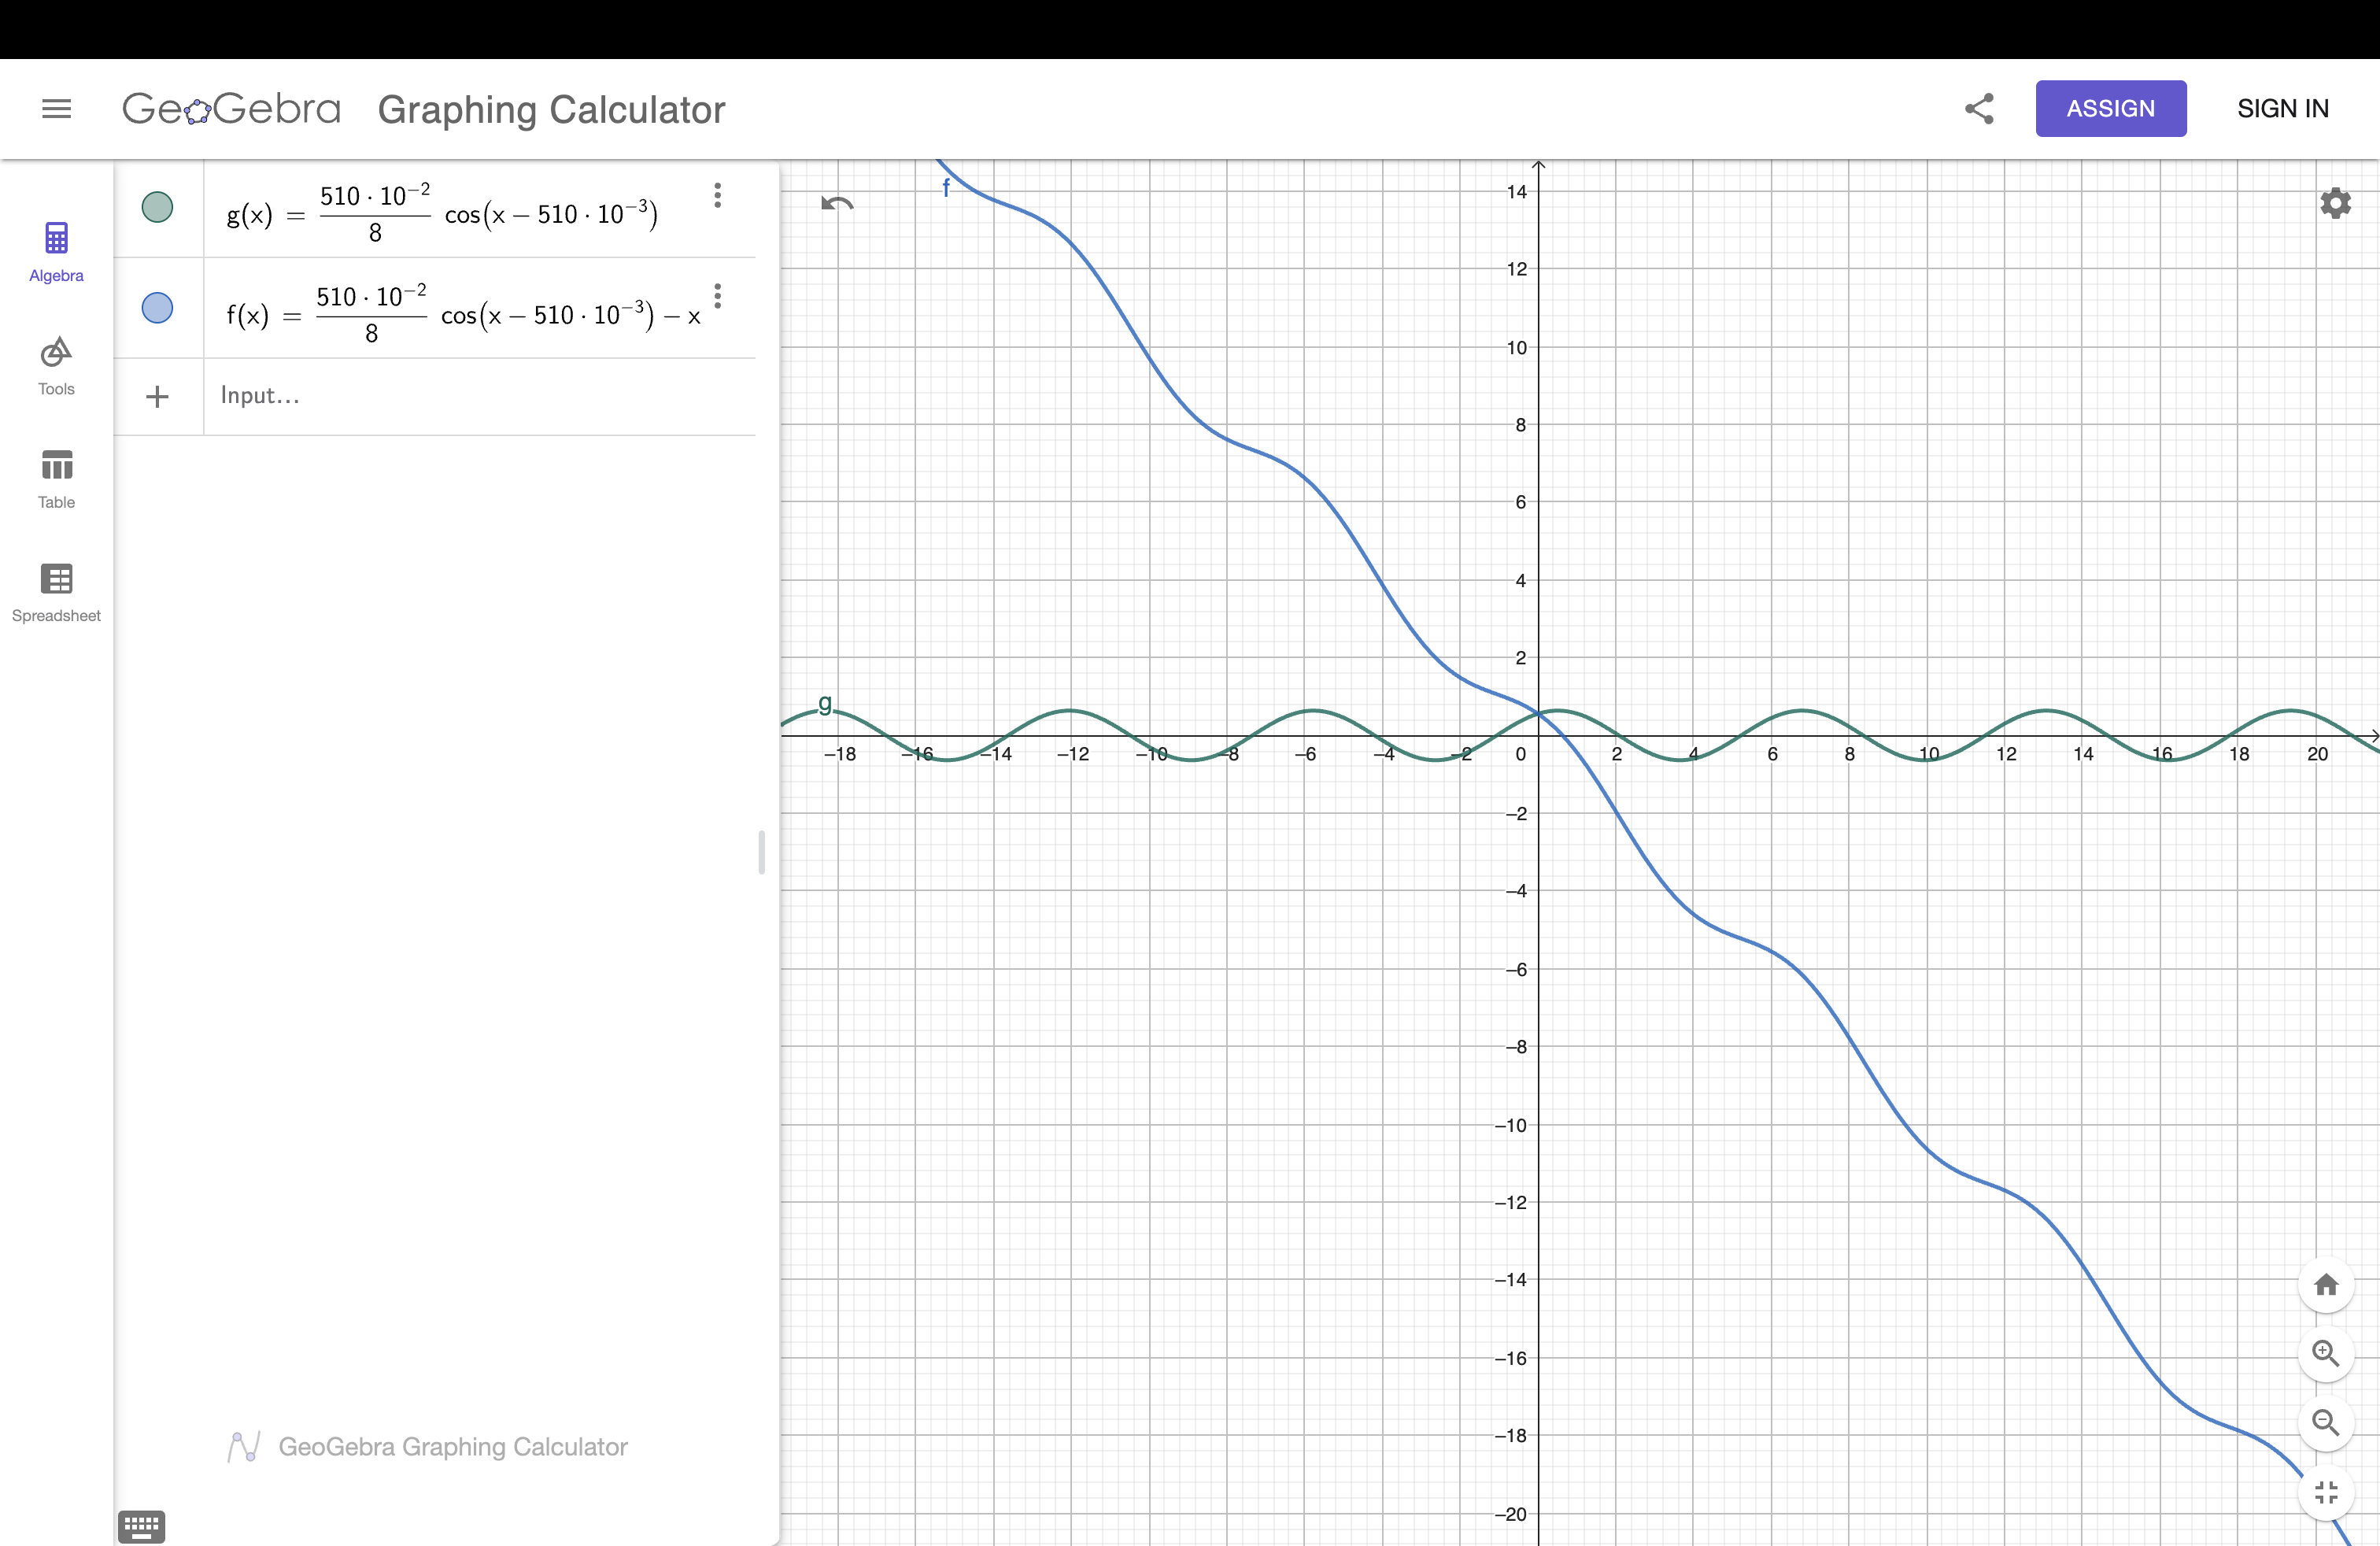
\includegraphics[width=\textwidth]{Figures/0. General/2.1.1.png}
        \caption{Gráfico de $f(x)$ y $g(x)$}
        \label{fig: Grafico de f(x) y g(x)}
    \end{subfigure}
\end{figure}

\subsection{Gráfico de $f(x)$ y $g(x)$ con intervalo $[0,2]$}
\begin{figure}[H]
    \centering
    \begin{subfigure}[b]{\textwidth}
        \centering
        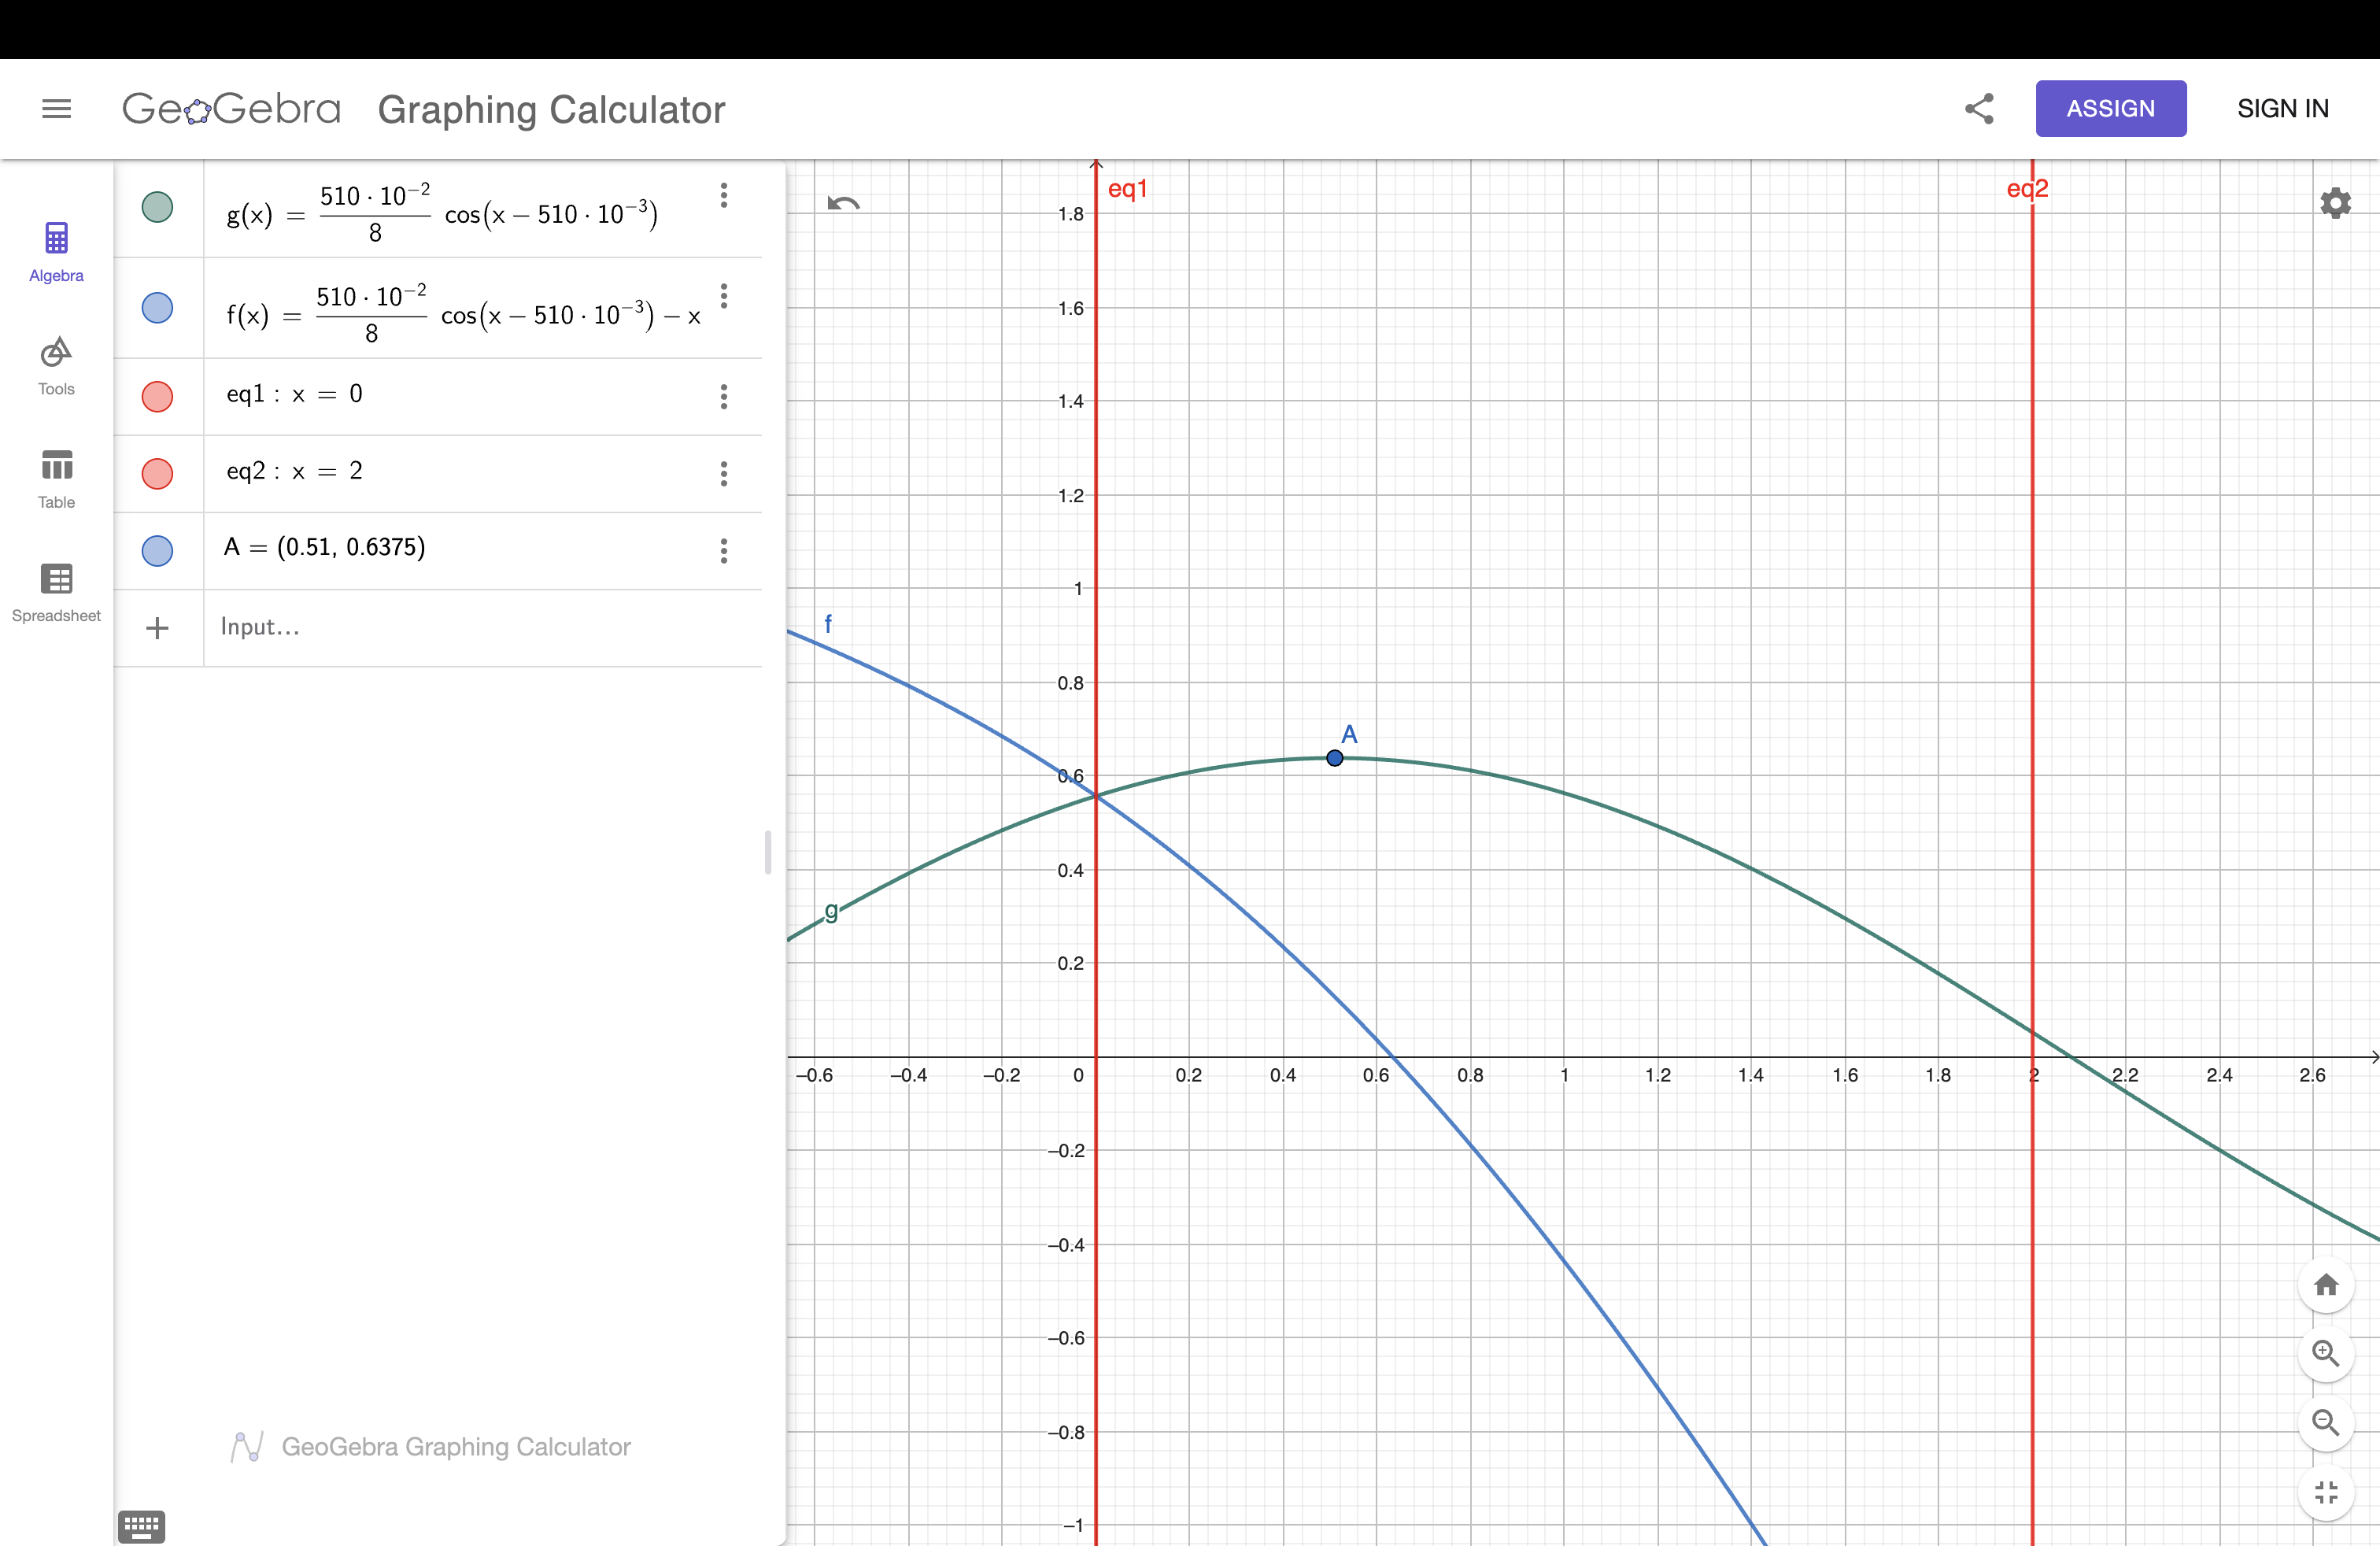
\includegraphics[width=\textwidth]{Figures/0. General/2.1.2.png}
        \caption{Gráfico de $f(x)$ y $g(x)$ con intervalo $[0,2]$}
        \label{fig: Grafico de f(x) y g(x) con intervalo [0,2]}
    \end{subfigure}
\end{figure}

\subsection{Análisis Gráfico en el intervalo \([0,2]\)}

Para que el método de punto fijo converja en un intervalo dado, se acostumbra verificar tres condiciones:

\begin{enumerate}
  \item \textbf{Continuidad de \(g(x)\) en \([0,2]\).}
  En la Figura \ref{fig: Grafico de f(x) y g(x)} y \ref{fig: Grafico de f(x) y g(x) con intervalo [0,2]}, puede apreciarse que \(g(x)\) (curva verde) es continua en el rango mostrado, pues está definida para todos los \(x\) entre 0 y 2.

  \item \textbf{Auto-mapeo:} \(g(x)\) debe enviar valores de \([0,2]\) de vuelta a \([0,2]\).
  Gráficamente, esto se observa si, para todo \(x\in[0,2]\), la imagen \(g(x)\) (altura en el eje \(y\)) se encuentra también entre 0 y 2. Se puede verificar que:
  \[
    0 \;\le\; g(x) \;=\;0.6375 \,\cos(x-0.510) \;\le\;2
    \quad\text{para }x\in[0,2],
  \]
  al menos de forma aproximada revisando que el máximo de \(0.6375 \cos(\dots)\) en ese rango no supere 2 y no se haga negativa de manera drástica. En la gráfica, se ve que \(g(x)\) permanece por encima de 0 y por debajo de 1 alrededor de ese intervalo.

  \item \textbf{Condición de contracción:} \(\max_{x\in [0,2]} \lvert g'(x)\rvert < 1.\)
  Para \(g(x) = 0.6375\,\cos(x - 0.510)\), la derivada es
  \[
    g'(x) \;=\; -\,0.6375\,\sin\bigl(x - 0.510\bigr).
  \]
  El valor absoluto es \(\lvert g'(x)\rvert = 0.6375\,\lvert\sin(\dots)\rvert \le 0.6375 < 1\) para todo \(x\). Por ende, en \([0,2]\), se cumple \(\lvert g'(x)\rvert<1\).

\end{enumerate}

\noindent
\textbf{Conclusión gráfica:}  
Dado que las tres condiciones se satisfacen en \([0,2]\), existe un único punto de intersección entre la gráfica de \(y=g(x)\) y la recta \(y=x\). Dicho punto es precisamente la solución de \(x = g(x)\), lo que confirma la convergencia al valor hallado (\(x\approx 0.6327\)) y explica por qué el método de punto fijo funcionó correctamente en ese intervalo.


Por lo que Daredevil 